\documentclass[border=10pt]{standalone}
\usepackage{tikz}
\usetikzlibrary{matrix, positioning, fit, decorations.pathreplacing, calligraphy}
\usepackage{amsmath, amssymb}

\begin{document}

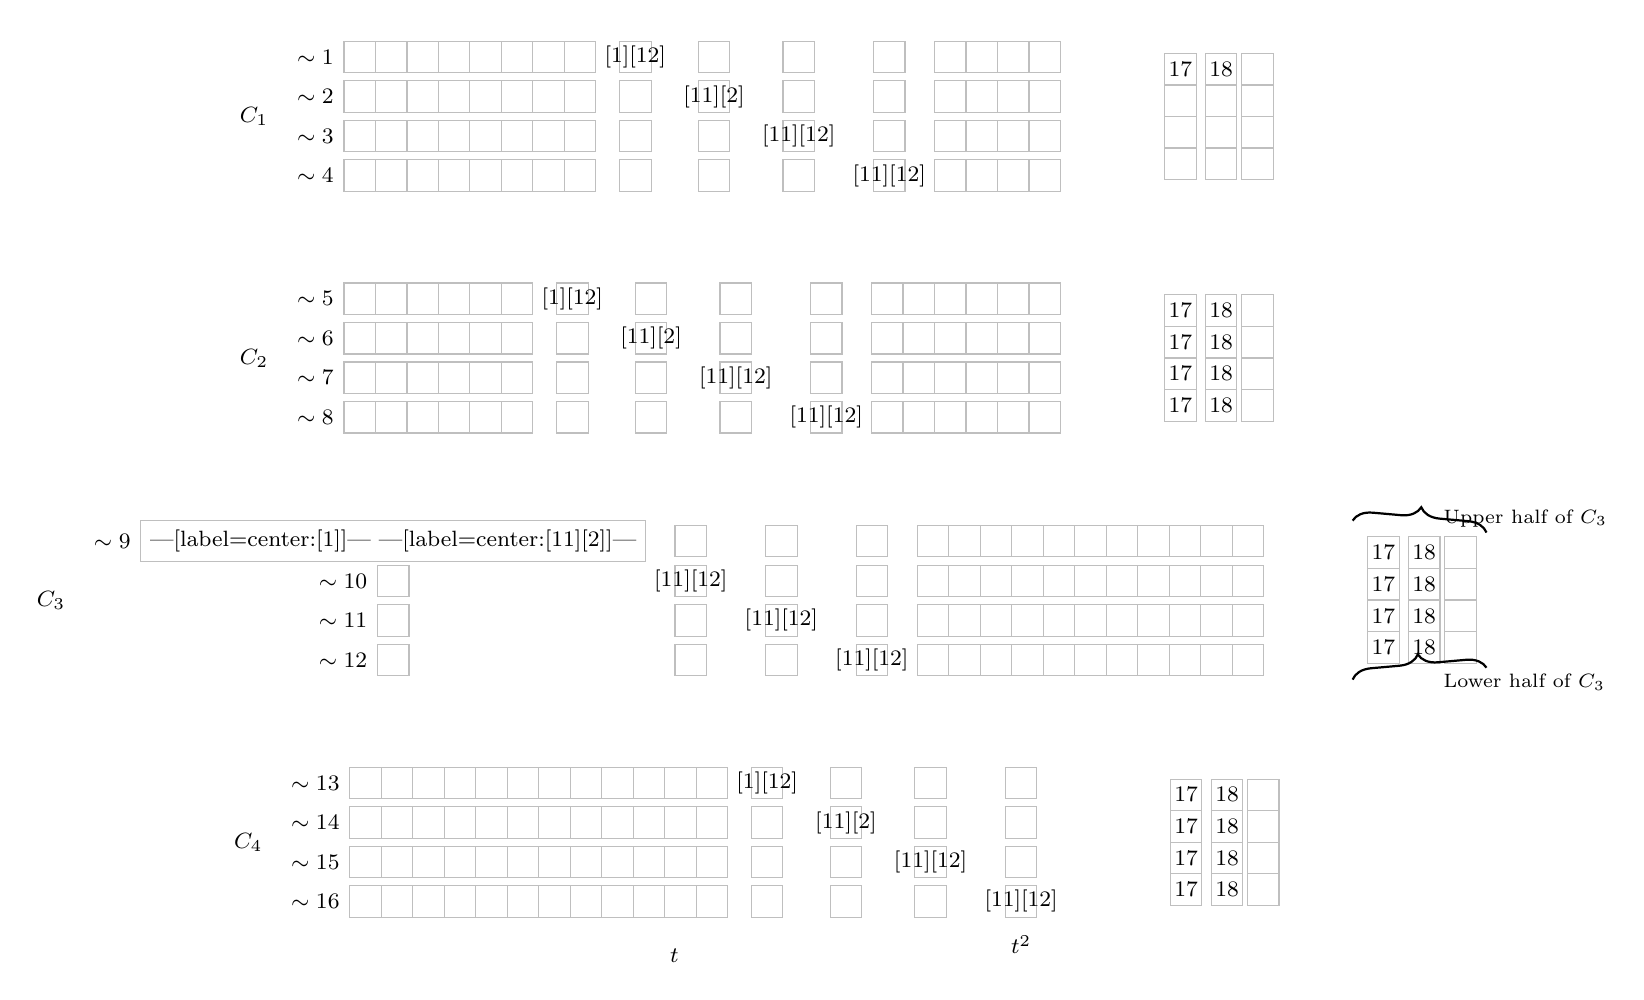
\begin{tikzpicture}[font=\footnotesize]
  % 定义样式
  \tikzset{
    grid cell/.style={
      minimum size=0.4cm,
      draw=gray!50,
      anchor=center,
    },
    matrix grid/.style={
      matrix of nodes,
      row sep=-\pgflinewidth,
      column sep=-\pgflinewidth,
      nodes={grid cell},
      nodes in empty cells
    },
    small matrix/.style={
      matrix of nodes,
      row sep=-\pgflinewidth,
      column sep=-\pgflinewidth,
      nodes={grid cell, minimum size=0.4cm},
      nodes in empty cells
    }
  }

  % C1 矩阵
  \matrix (C1) [matrix grid, label=left:$C_1$] {
    |[label={left:$\sim 1$}]| & & & & & & & & |[label={center:[1][12]}]| & & & & & & & \\
    |[label={left:$\sim 2$}]| & & & & & & & & & |[label={center:[11][2]}]| & & & & & & \\
    |[label={left:$\sim 3$}]| & & & & & & & & & & |[label={center:[11][12]}]| & & & & & \\
    |[label={left:$\sim 4$}]| & & & & & & & & & & & |[label={center:[11][12]}]| & & & & \\
  };

  % C2 矩阵
  \matrix (C2) [matrix grid, below=0.8cm of C1, label=left:$C_2$] {
    |[label={left:$\sim 5$}]| & & & & & & |[label={center:[1][12]}]| & & & & & & & & & \\
    |[label={left:$\sim 6$}]| & & & & & & & |[label={center:[11][2]}]| & & & & & & & & \\
    |[label={left:$\sim 7$}]| & & & & & & & & |[label={center:[11][12]}]| & & & & & & & \\
    |[label={left:$\sim 8$}]| & & & & & & & & & |[label={center:[11][12]}]| & & & & & & \\
  };

  % C3 矩阵
  \matrix (C3) [matrix grid, below=0.8cm of C2, label=left:$C_3$] {
    |[label={left:$\sim 9$}]| |[label={center:[1]}]| |[label={center:[11][2]}]| & & & & & & & & & & & & & & \\
    |[label={left:$\sim 10$}]| & |[label={center:[11][12]}]| & & & & & & & & & & & & & \\
    |[label={left:$\sim 11$}]| & & |[label={center:[11][12]}]| & & & & & & & & & & & & \\
    |[label={left:$\sim 12$}]| & & & |[label={center:[11][12]}]| & & & & & & & & & & & \\
  };

  % C4 矩阵
  \matrix (C4) [matrix grid, below=0.8cm of C3, label=left:$C_4$] {
    |[label={left:$\sim 13$}]| & & & & & & & & & & & & |[label={center:[1][12]}]| & & & \\
    |[label={left:$\sim 14$}]| & & & & & & & & & & & & & |[label={center:[11][2]}]| & & \\
    |[label={left:$\sim 15$}]| & & & & & & & & & & & & & & |[label={center:[11][12]}]| & \\
    |[label={left:$\sim 16$}]| & & & & & & & & & & & & & & & |[label={center:[11][12]}]| \\
  };

  % 右侧小矩阵
  \matrix (R1) [small matrix, right=1cm of C1] {
    |[label={center:17}]| & |[label={center:18}]| & \\
    & & \\
    & & \\
    & & \\
  };

  \matrix (R2) [small matrix, right=1cm of C2] {
    |[label={center:17}]| & |[label={center:18}]| & \\
    |[label={center:17}]| & |[label={center:18}]| & \\
    |[label={center:17}]| & |[label={center:18}]| & \\
    |[label={center:17}]| & |[label={center:18}]| & \\
  };

  \matrix (R3) [small matrix, right=1cm of C3] {
    |[label={center:17}]| & |[label={center:18}]| & \\
    |[label={center:17}]| & |[label={center:18}]| & \\
    |[label={center:17}]| & |[label={center:18}]| & \\
    |[label={center:17}]| & |[label={center:18}]| & \\
  };

  \matrix (R4) [small matrix, right=1cm of C4] {
    |[label={center:17}]| & |[label={center:18}]| & \\
    |[label={center:17}]| & |[label={center:18}]| & \\
    |[label={center:17}]| & |[label={center:18}]| & \\
    |[label={center:17}]| & |[label={center:18}]| & \\
  };

  % C3 的上半部分和下半部分标注
  \draw[decorate, decoration={brace, amplitude=7pt}, thick] 
    ([yshift=+0.5ex]R3.north west) -- node[right=5pt, yshift=3pt] {\scriptsize Upper half of $C_3$} ([yshift=-0.5ex]R3.north east);
  \draw[decorate, decoration={brace, amplitude=7pt}, thick] 
    ([yshift=-0.5ex]R3.south west) -- node[right=5pt, yshift=-3pt] {\scriptsize Lower half of $C_3$} ([yshift=+0.5ex]R3.south east);

  % 底部标签
  \node[below=0.1cm of C4] {$t$};
  \node[below=0.1cm of C4-4-16] {$t^2$};

\end{tikzpicture}

\end{document}